\section{Models}
Now the feature vectors are extracted we can begin to develop classification models. In this section I will briefly go through the theory of for classic machine learning models and continue to explain the core concepts of the neural network architectures

The problem of assigning one of mutually exclusive languages to a sentence is an example of a multi class classification problem. Since we have gathered a dataset with which we can train our models we are dealing with supervised learning.

Let us start with developing a bit of notation.
We are provided with a set of data points $\mathcal{X}$ together with an associated set of labels $\mathcal{Y}$.
We can define our \emph{dataset} $\mathcal{D}$ the as follows
\begin{align}
\mathcal{D} = \{(\mathbf{x}_i,y_i)|\mathbf{x}_i\in\mathcal{X},y_i\in\mathcal{Y}\}
\end{align}

where we have that the data points and labels are defined by
\begin{align}
\mathcal{X}&=\{\mathbf{x}_1, \mathbf{x}_2, \mathbf{x}_3, \cdots,\mathbf{x}_n\} \qquad \mathbf{x}_i \in \mathbf{R}^{m}  \\
\mathcal{Y}&=\{y_1, y_2, y_3, \cdots,y_n\} \qquad y_i \in C
\end{align}
Where $C$ is the set of possible language categories, in this case the set
\begin{align}
  C = \{"dk", "sv", "nn", "nb", "fo", "is"\}
\end{align}
Now our aim is to construct a function $f$ of some parameters $\theta$ such that given a datapoint $\mathbf{x}$ the function returns the predicted label $\hat{y}$

\begin{align}
 \hat{y} = f_\theta (\mathbf{x})
\end{align}

Now the predicted label might not be correct and we need a measure of how wrong our model is over the whole dataset. One common error function is the mean squared error (MSE) cost function.

\begin{align}
  E_{\text{MSE}} = \frac{1}{n}\sum_i^n (\hat{y}_i - y_i)^2
\end{align}
Later for the training of the neural networks with keras we will use the categorical cross entropy (CCE) which is given by.
\begin{align}
  E_{\text{CCE}} = -\frac{1}{n}\sum_i^n \sum_{c\in C} y_{i,c}\ln \hat{y_{i,c}}
\end{align}

\subsection{Baseline models}

As mentioned in \cite{BagOfTricks}, simple baseline models for text classification are for example logistic regression and support vector machines. In this project I will also test how the performance of the K Nearest Neighbors algorithm and a Naive Bayes classifier.
%
% In addition to the neural networks I would like to test how more conventional Machine Learning models compare to models based on neural networks.

\subsubsection{K Nearest Neighbors}
Perhaps the simplest model to understand is the K Nearest Neighbors classification algorithm. Here we calculate the distance from a test example which we want to label to its $k$ "Nearest Neighbors". The distance $d$ between the test example $\mathbf{x}$ and a labeled data point $\mathbf{x}_{\text{train}}$ in the training set is the conventional euclidean distance.

\begin{align}
d=\sqrt{\sum_{i=1}^m (x_i-x_{\text{train}_i})^2}
\end{align}

The algorithm calculates the distance $c$ between a test point $\mathbf{x}$ to all other data points in the training set. Then we simply assign the most common label to $\mathbf{x}$ among its $k$ nearest neighbors. In this project and for the results to be presented later we have set $k=3$.

\subsubsection{Linear support vector machines}
Support vector machine is all about finding the maximal margin hyperplanes.

Any hyper plane in the feature space can be written as points satisfying
\begin{align}
    \mathbf{w}\cdot\mathbf{x} + \mathbf{b} = 0
\end{align}

We want to find the two parallel hyperplanes where the distance between them is at large as possible.
The functional form of the linear support vector machine then becomes
\begin{align}
    \hat{y} = \text{sign}(\mathbf{w}\cdot \mathbf{x} + b)
\end{align}
Where we define
\begin{align}
    \mathbf{w} = \sum_i \alpha y_i \mathbf{x}_i
\end{align}
Where $\alpha_i$ is only non-zero for the support  vectors $\mathbf{x}_i$. Thus the aim thus the aim is to minimize $||\mathbf{w}||$ since the width between the two supporting hyperplanes is proportional to $1/||\mathbf{w}||$

\subsubsection{Logistic Regression}
Contrary to the k nearest neighbors and support vector machine algorithm described above in Logistic regression we calculate the probability that $\mathbf{x}$ belongs to the language $C_k$ as
\begin{align}
p(C_k|\mathbf{x}) = f(\mathbf{x}) = \frac{1}{1+e^{\theta^T \mathbf{x}}}
\end{align}
The predicted label of the logistic regression model is then given by
\begin{align}
  \hat{y} = \text{argmax}_k p(C_k|\mathbf{x})
\end{align}
The method for finding the parameters $\theta$ which minimizes the error is gradient decent which is given by
\begin{align}
  \theta_{t+1} = \theta_t + \eta \nabla E
\end{align}

\subsubsection{Naive Bayes}
% Our goal is to find the probability of belonging to a language class $C_k$. given a sentence $\mathbf{x}$ $p(C_k|\mathbf{x})$.  The famous Bayes' theorem states that
%
% \begin{align}
% p(A|B) = \frac{p(B|A)p(A)}{p(B)}
% \end{align}

Our goal is to find the probability of belonging to a language class $C_k$. We can use Bayes' theorem here to find the probability $p(C_k|\mathbf{x})$ of a language class $C_k$ given a feature vector $\mathbf{x}$. Using Bayes Theorem we get

\begin{align}
p(C_k|\mathbf{x}) = \frac{p(C_k)}{p(\mathbf{x})} p(\mathbf{x}|C_k)
\label{bayes1}
\end{align}

Now the prior $p(\mathbf{x})$ is a constant and so it $p(C_k)$ if the number of data points in each of the language categories are equal, as is the case here. We can rewrite $p(\mathbf{x}|C_k)$ using the assumption that the features $x_i$\footnote{This is the "naive" part of Naive Bayes} are independent we can write.
\begin{align}
p(\mathbf{x}|C_k) = p(C_k) \prod_i p(x_i|C_k)
\label{bayes2}
\end{align}
By using eq. $\ref{bayes2}$ in eq. $\ref{bayes1}$ and selecting the largest probability we get the prediction by.

\begin{align}
\hat{y} = \underset{k}{\text{argmax  }} p(C_k) \prod_i p(x_i|C_k)
\end{align}
% \begin{align}
% p(C_k|\mathbf{x}) \propto p(C_k) \prod_i p(x_i|C_k)
% \end{align}

\subsection{Neural Networks}
In this section I will go through the basic theory behind the two neural network architectures Multi layer Perceptrons and convolutional neural networks.


\subsubsection{Feed Forward Neural Networks}
Arguably the simplest neural network if the Multi Layer Perception MLP. A MLP consists of at least 3 layers where the first is the input layer which have the same number of nodes as the feature vector we feed into the network. The last layer is the output layer which always have the same number of nodes at the number of different classes, six in this cave.

In the MLP we use dense layers as the hidden layers, this means that all the nodes in a layer are connected to all nodes in the next layer.

In each layer we take the output from the previous layer and multiply each component with a set of weights, the values of which we optimize during training, sum them up and pass the result to a nonlinear activation function.

The activation function in the hidden layers is the rectified linear unit or ReLU function
\begin{align}
  \text{ReLU}(z)= \text{max}(0,z)
\end{align}

The activation function final layer is the softmax function
\begin{align}
  \text{softmax}(z)_i= \frac{e^z_i}{\sum_{j=1}^k e^z_j}
\end{align}
where $k$ is the number of different classes.

\subsubsection{Convolutional Neural Networks}

While every layer in the MLP is densely connected such that each of the nodes in a layer is connected to all nodes in the next layer, in a convolution neural network we use one or more convolutional layers.

Convolutional Neural networks are very popular for image recognition but they can also be used for text classification \cite{textcnn_google}.

\begin{figure}[h!]
  \centering
  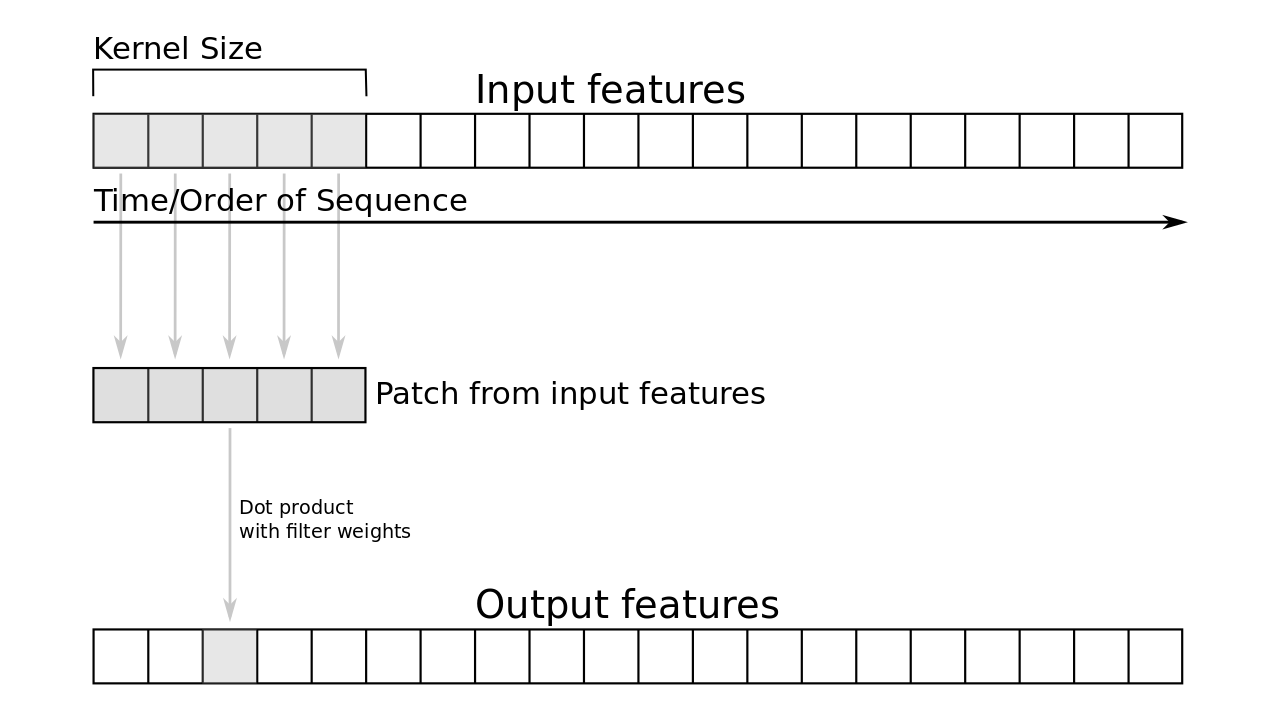
\includegraphics[width = 200pt]{figs/cnn_diagram}
  \caption{Diagram of Convolutional Neural network.}
  \label{cnn}
\end{figure}

The basic premise of a convolutional layer is illustrated in figure \ref{cnn}\footnote{Source: \url{https://realpython.com/python-keras-text-classification/}}. In a CNN you have a filter which slides over the input. The CNN then takes the dot product of the weights of the filter and the corresponding input features, before applying the activation function. The kernel size is a hyper parameter which can be optimized by experimentation which we will also do later.

